% author: Andreas Kelbel
%
\documentclass{standalone}
% packages
	\usepackage{tikz}
		\usetikzlibrary{decorations.pathmorphing,patterns}
	\usepackage{cmbright}		% font 
%
\begin{document}
  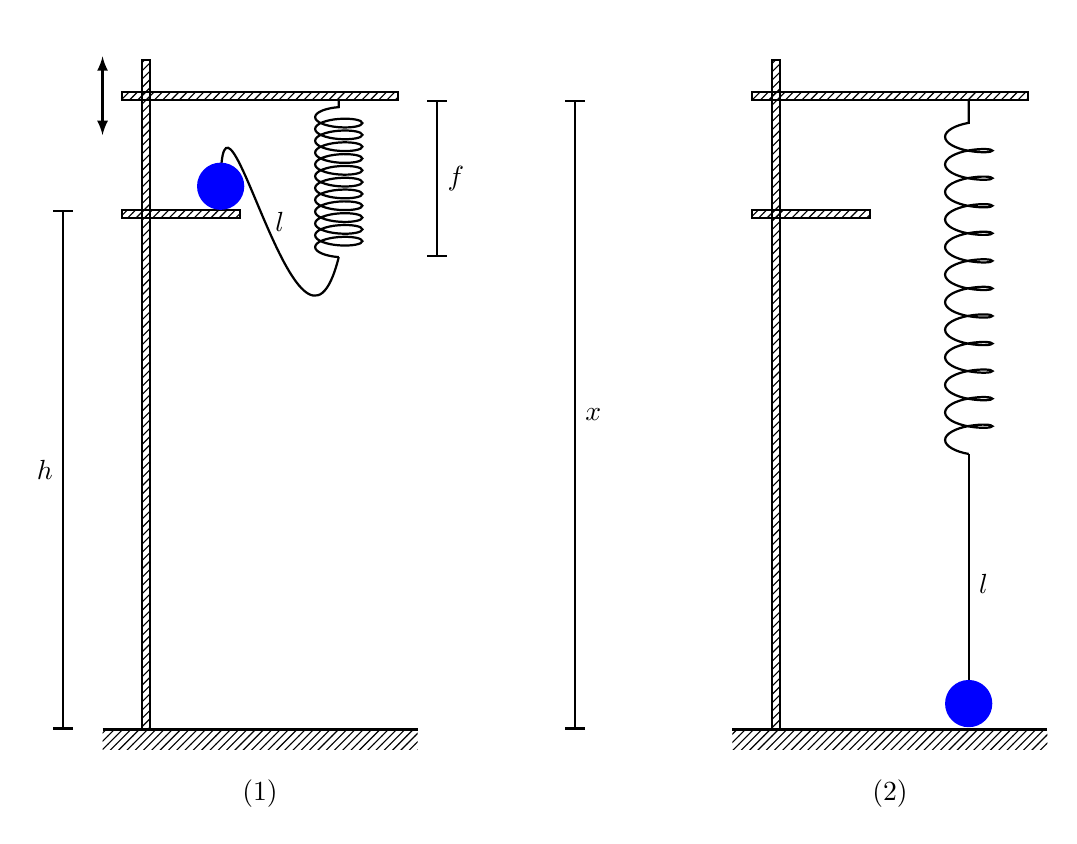
\begin{tikzpicture}
	\begin{scope}[thick]
      \fill [pattern = north east lines] (0,0) rectangle (4,-.25);
      \draw (0,0) -- (4,0);
      \draw (2,-.5) node[below]{(1)} ;
      \filldraw[pattern = north east lines] (.5,0) rectangle ++(.1,8.5) ;
      \filldraw[pattern = north east lines] (.25,8) rectangle ++(3.5,.1) ;
      \filldraw[pattern = north east lines] (.25,6.5) rectangle ++(1.5,.1) ;
      \draw (1.5,6.9) .. controls +(0,2) and +(-.5,-2) .. (3,6) node[midway,right]{$l$} ;
      \fill[blue] (1.5,6.9) circle (3mm) ;

      \draw[decoration={aspect=0.3, segment length=1.5mm, amplitude=3mm,coil},decorate] (3,6) -- (3,8) ; 
      \draw[|-|] (-.5,0) -- +(0,6.6) node[midway, left]{$h$};
      \draw[|-|] (4.25,6) -- +(0,2) node[midway, right]{$f$};
      \draw[|-|] (6,0) -- +(0,8) node[midway, right]{$x$};
      \draw[latex-latex] (0,7.55) -- +(0,1) ;
      \end{scope}
      \begin{scope}[thick,xshift=8cm]
      \fill [pattern = north east lines] (0,0) rectangle (4,-.25);
      \draw (0,0) -- (4,0);
      \draw (2,-.5) node[below]{(2)} ;
      \filldraw[pattern = north east lines] (.5,0) rectangle ++(.1,8.5) ;
      \filldraw[pattern = north east lines] (.25,8) rectangle ++(3.5,.1) ;
      \filldraw[pattern = north east lines] (.25,6.5) rectangle ++(1.5,.1) ;
      \draw (3,3.5) -- (3,.2) node[midway,right]{$l$} ;
      \fill[blue] (3,.33) circle (3mm) ;

      \draw[decoration={aspect=0.3, segment length=3.5mm, amplitude=3mm,coil},decorate] (3,3.5) -- (3,8) ; 
	\end{scope}
  \end{tikzpicture}
\end{document} 